% compile with: pdflatex -shell-escape filename.tex
\documentclass[convert=pdf2svg]{standalone}
\usepackage{tikz}
\usetikzlibrary{patterns,positioning}

\tikzset{
  every node/.style = {font=\Large},
  point/.style = { circle, fill, inner sep=2.5pt },
}

\begin{document}
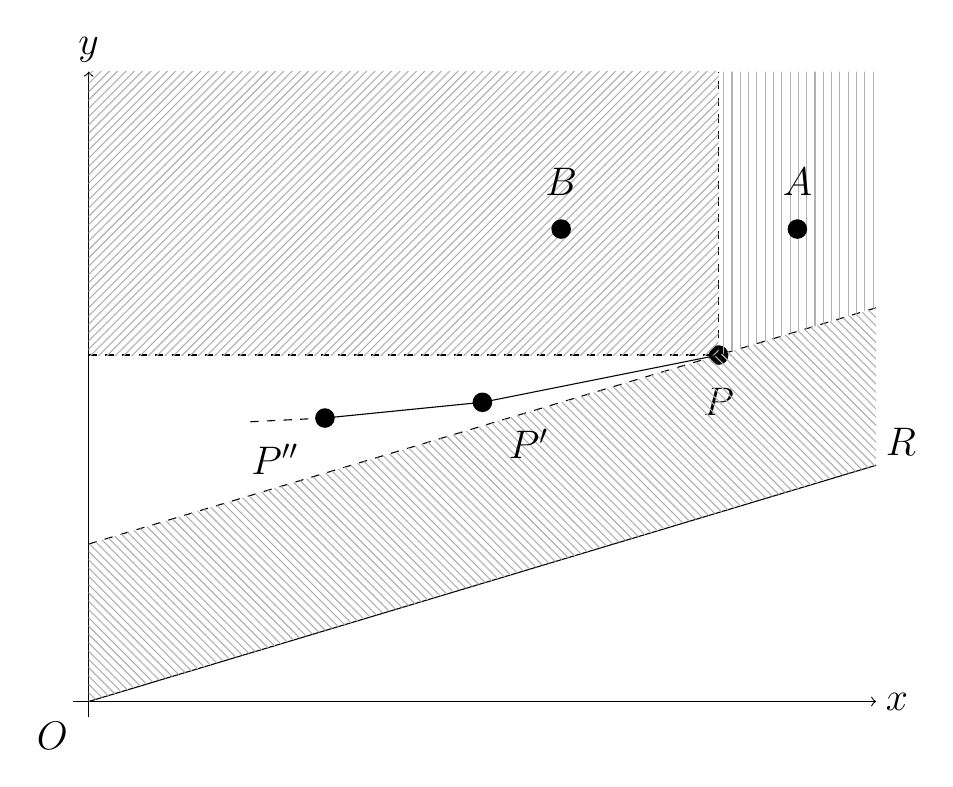
\begin{tikzpicture}[label distance=3mm]

  % coordinate system
  \draw[->] (-0.2,0) -- (10,0) node[right]{$x$};
  \draw[->] (0,-0.2) -- (0,8) node[above]{$y$};
  \node at (0,0) [below left=2mm] {$O$};

  % ray R and point P
  \draw (0,0) -- (10,3) node[above right]{$R$};
  \coordinate[label=below:$P$] (P) at (8,4.4);
  \node at (P)[point] {};

  % dashed lines through P
  \draw[dashed] (0,2) -- (10,5);
  \draw[dashed] (0,4.4) -- (P);
  \draw[dashed] (P) -- (8,8);

  % areas where no candidate points can exist
  \fill [pattern={north east lines}, pattern color=black!30]
    (0,4.4) rectangle (8,8);
  \fill [pattern={vertical lines}, pattern color=black!30]
    (8,4.4) -- (10,5) -- (10,8) -- (8,8);
  \fill [pattern={north west lines}, pattern color=black!30]
  (0,0) -- (10,3) -- (10,5) -- (0,2);

  % other candidate points
  \coordinate[label=below right:$P'$] (P2) at (5,3.8);
  \node at (P2)[point] {};
  \coordinate[label=below left:$P''$] (P3) at (3,3.6);
  \node at (P3)[point] {};
  \draw (P) -- (P2) -- (P3);
  \draw[dashed] (P3) -- (2, 3.55);

  % bad points which can never be the answer due to P's existence
  \coordinate[label=above:$A$] (A) at (9,6);
  \node at (A)[point] {};
  \coordinate[label=above:$B$] (B) at (6,6);
  \node at (B)[point] {};
\end{tikzpicture}

\end{document}
